\RequirePackage{luatex85}
\documentclass[amsmath]{article}
\usepackage{amsmath}
\usepackage{amssymb}
\usepackage{geometry,contour}
\usepackage{tikz}
\usetikzlibrary{shapes,snakes}
\usetikzlibrary{shapes.geometric, arrows}
\usetikzlibrary{decorations.text}

\geometry{legalpaper, landscape, top=0.1in, left=0in, right=0in}
\paperheight 2in
\paperwidth 4.3in

\begin{document}
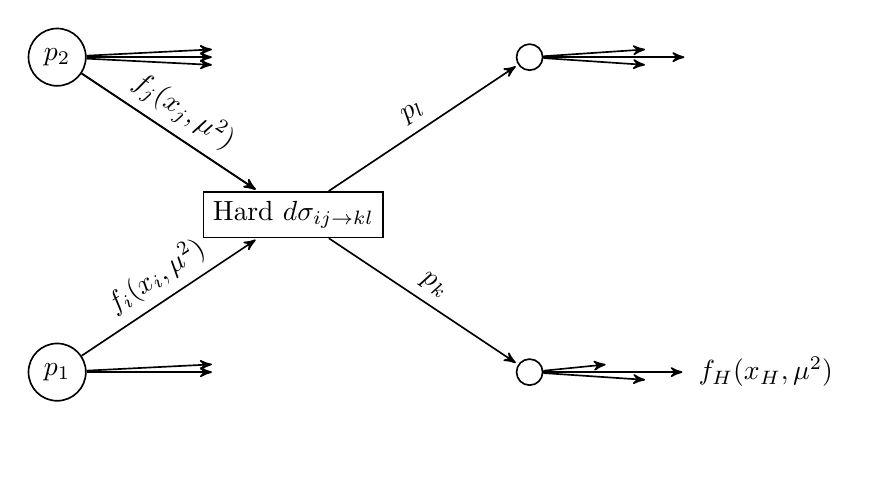
\begin{tikzpicture}[
  ->,
  >=stealth',
  shorten >=1pt,
  auto,
  node distance=2.8cm,
  semithick,
  every state/.style={fill=red,draw=none,text=white},
]
\node[draw, circle] (A) at (0,0) {$p_1$}; 
\node[draw, circle] (B) at (0,4) {$p_2$}; 
\node[draw, circle] (C) at (6,0) {}; 
\node[draw, circle] (D) at (6,4) {}; 
\node[draw, rectangle] (V) at (3,2) {Hard $d\sigma_{ij\rightarrow kl}$}; 
\path[every node/.style={sloped,anchor=south,auto=false}]
        (A) edge node {$f_{i}(x_i, \mu^2)$} (V)            
        (B) edge  node {$f_{j}(x_j, \mu^2)$} (V)
        (V) edge node {$p_k$} (C)            
        (V) edge  node {$p_l$} (D);
\draw[->] (A) edge (2,0);
\draw[->] (A) edge (2,0.1);
\draw[->] (B) edge (V);
\draw[->] (B) edge (2,3.9);
\draw[->] (B) edge (2,4);
\draw[->] (B) edge (2,4.1);

\node[circle] (F) at (9,0) {$f_{H}(x_H, \mu^2)$}; 
\draw[->] (C) edge (F); 
\draw[->] (C) edge (7.5,-.1); 
\draw[->] (C) edge (7,.1); 
\draw[->] (D) edge (7.5,3.9);
\draw[->] (D) edge (8,4);
\draw[->] (D) edge (7.5,4.1);


\end{tikzpicture}
\end{document}